\newpage
\section{Einleitung}
\label{sec:Einleitung}

\subsection{Vorstellung des Projektes}
\label{sec:Vorstellung des Projektes}
Im Rahmen der Veranstaltung \textit{Frameworkbasierte GUI-Entwicklung} wurde das Projekt \textit{HeartRate2Go} ausgearbeitet. \textit{HeartRate2Go} ist ein Softwarepaket bestehend aus einer Desktop-PC Anwendung und einem Android Smartphone/Smartwatch App-Bundle zur Erfassung der Herzfrequenz für Ruhe- oder Aktivitätsmessungen. Die von der Smartwatch per Pulsoxymetrie gemessenen Herzfrequenz wird über das gekoppelte Smartphone zur Desktop-PC Anwendung übertragen und dort übersichtlich zusammen mit bereits getätigten Messungen dargestellt. \textit{HeartRate2Go} unterstützt damit den Anwender bei der Kontrolle seines Pulses, auch über längere Zeiträume hinweg.

\subsection{Ablauf einer Messung}
%Ablauf einer Messung, vllt mit Diagramm 
%Anwender trägt Uhr, startet App, wählt Messart aus, Messung startet, evtl Messung beenden, Abfrage über Stimmung, Smartphone zeigt Durchschnittswert an, Smartphone empfängt Daten automatisch von der Uhr, Smartphone zeigt Werte im Balkendiagramm an, GUI öffnen, GUI empfängt Messdaten per tcp über Smartphone (wird vom Smartphone gesteuert), Messdaten werden in GUI eingefügt und graphisch dargestellt, Messwerte können mit vergangen Messungen verglichen und auch gedruckt werden.

Um \textit{HeartRate2Go} verwenden zu können sind zunächst drei Hardware-Komponenten notwendig:
\begin{itemize}
	\item Eine Android-Smartwatch
	\item Ein Android-Smartphone und
	\item Ein Desktop-PC (mit Windows, Linux oder OS X)
\end{itemize}


\begin{figure} [H]
	\centering
		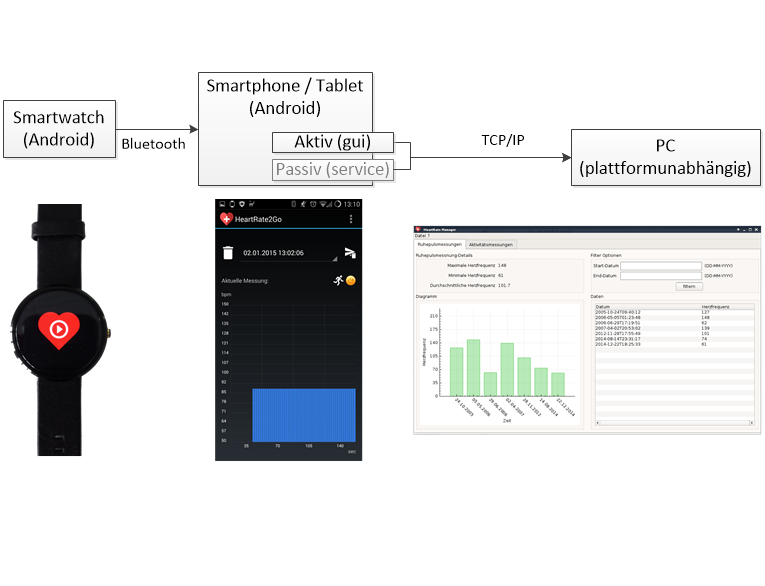
\includegraphics[scale=0.68]{images/ablauf.png}
		\caption{Ablauf der Datenübertragung}
		\label{fig:ablauf}
\end{figure}

Für eine Messung trägt der Anwender die Smartwatch am Handgelenk und startet die \textit{HeartRate2Go}-App. Er wählt nun aus, ob er eine Ruhe- oder eine Aktivitätsmessung durchführen möchte. Anschließend wird der Messvorgang gestartet. Bei einer Ruhemessung wird die Messung automatisch nach einer festgelegten Zeit beendet, bei der Aktivitätsmessung muss der Benutzer die Messung manuell beenden. 
Nach Abschluss des Messvorgangs wird der Anwender nach seiner Stimmung während der Messung gefragt. Er kann zwischen ''gut'', ''okay'' und ''schlecht'' wählen. Die Übertragung der Messwerte von der Smartwatch an das gekoppelte Smartphone wird automatisch per Bluetooth durchgeführt, sobald sich das Smartphone in Reichweite befindet. Auf der Smartphone-App werden dann die Messungen bereits in einem vorläufigen Balkendiagramm angezeigt. Der Anwender ist dann jederzeit in der Lage die auf dem Smartphone gespeicherten Messungen über das Heimnetzwerk per Knopfdruck an die PC-Anwendung zu übertragen. In Abbildung \ref{fig:ablauf} ist der Ablauf der Datenübertragung nochmals visualisiert.

\subsection{Medizinische Apps}
\label{sec:Medizinische Apps}
Im Laufe der letzten Jahre wurde der Markt mit Apps, die einen medizinischen Hintergrund besitzen, überschüttet. Wenn man im deutschen iTunes-Store nach „Medizin“ sucht, erhält man mehrere hundert Einträge, dies gilt genauso für den Google-Play Store. \\[0.5cm]
Im vergangen Jahr sind die Absatzzahlen von medizinischen Apps in Großbritannien, Frankreich, Niederlande und Deutschland um 42 Prozent gestiegen, vermeldet das GfK (Marktforschungszentrum).\\
Diese Apps decken nahezu jeden Bereich der Medizin ab, egal ob es um die Speicherung von Vitaldaten, die Messung von Vitaldaten mit einem zusätzlichen Messgerät und die Auswertung der Daten geht. Des Weiteren sind auch viele Nachschlagewerke darunter enthalten.\\[0.5cm]
Zu beachten ist allerdings, dass keiner der Apps den Arztbesuch ersetzt. Sie geben lediglich eine erste Einschätzung und sind dadurch eine große Erleichterung für den Nutzer. Allerdings ist es auch so, dass jeder Programmierer eine App mit medizinischem Hintergrund in die verschiedenen Stores hochladen darf. Diese werde nicht auf ihren Nutzen hin überprüft, so sind auch viele Apps zu finden, die mehr als Spielerei gelten.\\[0.5cm]
Kaum eine App ist ein Medizinprodukt nach dem Medizinproduktegesetzt, sie gelten lediglich als Wellness- beziehungsweise Lifestyle-Apps.
%Thema und Zielsetzung: Stellen Sie zunächst Thema und Zielstellung der Arbeit vor.
%Theorie: Vermitteln Sie Ihre Theorie(n) über das Thema und geben Sie an, auf was sich Ihre Theorie stützt.
%Fragestellung: Teilen Sie mit, welche Fragen in der folgenden Arbeit beantwortet werden.
%Quellen: Welche Quellen haben Sie für Ihre Arbeit genutzt bzw. wie haben Sie Ihre Frage(n) beantwortet?
%Ergebnis: Führen Sie Ihre Ergebnisse auf, also teilen Sie mit, was Sie herausgefunden haben.
%Fazit: Stellen Sie am Ende des Abstracts eine Quintessenz auf. Sie können Ihr Fazit auch mit einer %Zukunftsprognose verbinden.

\newpage
\subsection{Medizinische Kenntnisse - Pulsoxymetrie} 
Für die Messung des peripheren Pulses per Android-Uhr wird das Prinzip der Reflexions-Pulsoxymetrie genutzt (Abbildung \ref{pic:pulsoxy}).\\[0.5cm]
Dieses Verfahren benötigt zwei Sensoren: zum einen eine Lichtquelle, zum anderen ein Lichtsensor. Die Lichtquelle sendet Infrarot-Lichtwellen aus, die durch die Haut dringen. Der Sensor misst die Lichtanteile, die absorbiert wurden. \\[0.5cm]
Die Lichtabsorption im Blut ist abhänig von der Hämoglobinkonzentration und der Sättigung des Hämoglobins mit Sauerstoff. Oxigeniertes und desoxigeniertes Hämoglobin schwächen das Licht jeweils charakteristisch ab. \\[0.5cm]
Mit diesem Prinzip ist es auch möglich, die Sauerstoffsättigung im kapillären Blut zu messen \cite{behandlungsassitenz}.\\[0.5cm]
\begin{figure}[H]
	\centering
	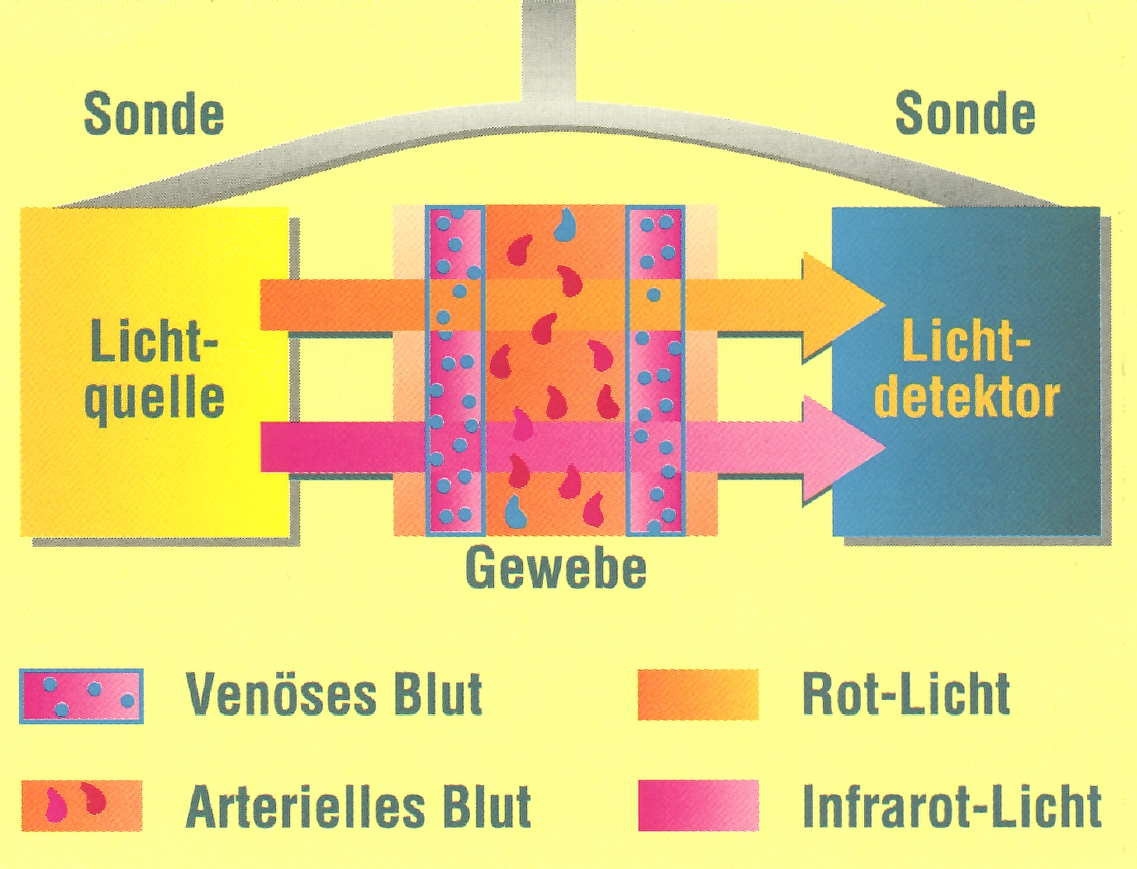
\includegraphics[scale=1.0]{images/pulsoxy.jpg}
	\caption{Veranschaulichung der Pulsoxymetrie\cite{messprinzip-pulsoxi}}
	\label{pic:pulsoxy}
\end{figure}


